\chapter{The Robot Software System (LabVIEW)}

\section{The FPGA Hindbrain}
As discussed in the software overview chapter, the Hindbrain of the vehicle is implemented on a LabVIEW FPGA in order to ensure that control loops and essential data processing is done at the fastest possible speeds to reduce system latency even when the vehicle travels at higher speeds. \\ \\
%
The front panel and block diagram of the top-level hindbrain VI is shown below:

\begin{figure}[h!]
\centering
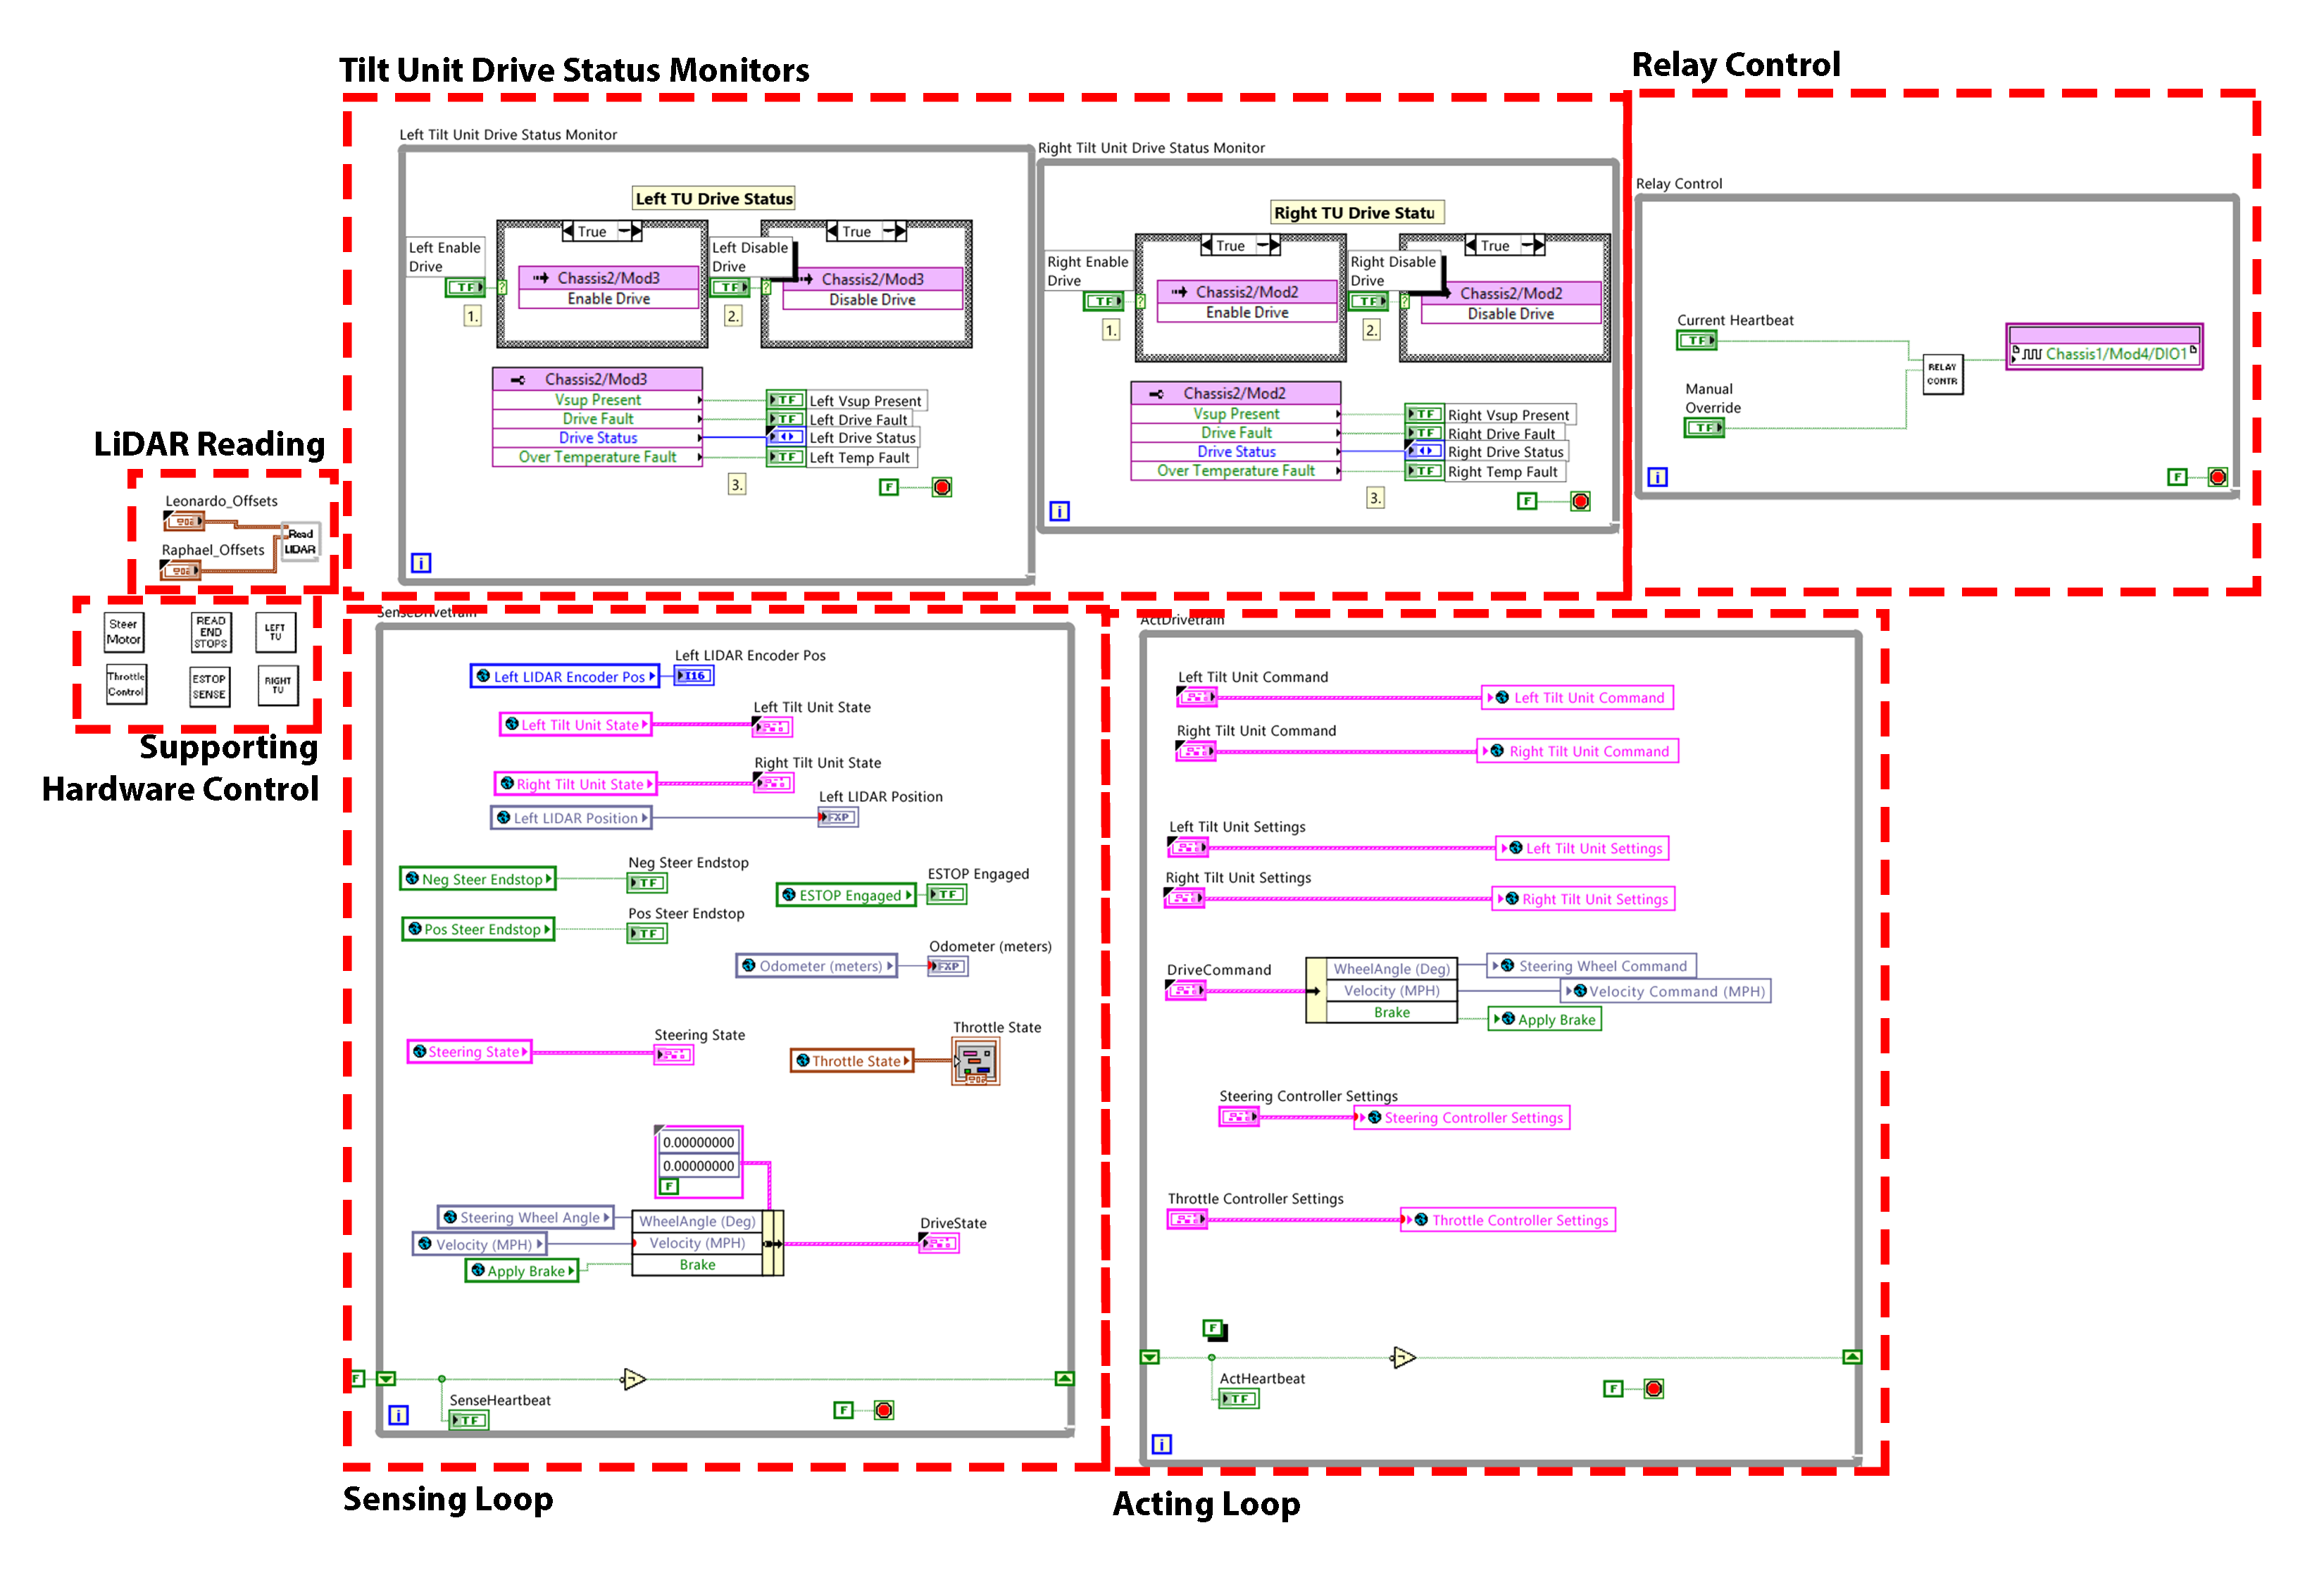
\includegraphics[scale=0.55]{Photos/hindbrainblock_annotated.png}
\caption{Hindbrain top-level VI block diagram with subchapters annotated}
\label{fig:hindbrainblock}
\end{figure} 

\newpage

\noindent As can be seen in Figure \ref{fig:hindbrainblock}, the main subchapters of the FPGA hindbrain are:

\begin{enumerate}
\item Sensing Loop
\item Acting Loop
\item Tilt Unit Drive Status Monitors
\item LiDAR Reading
\item Supporting Hardware Control
\item Relay Control
\end{enumerate}

\subsection{Sensing Loop}

The sensing loop of the FPGA hindbrain essentially passes status information and data from other parts of the FPGA hindbrain code up to the front panel so that the real-time code can access these variables. The block diagram for the sensing loop shown in Figure \ref{fig:hindbrainblock} is shown zoomed in below: 

\newpage

\begin{figure}[h!]
\centering
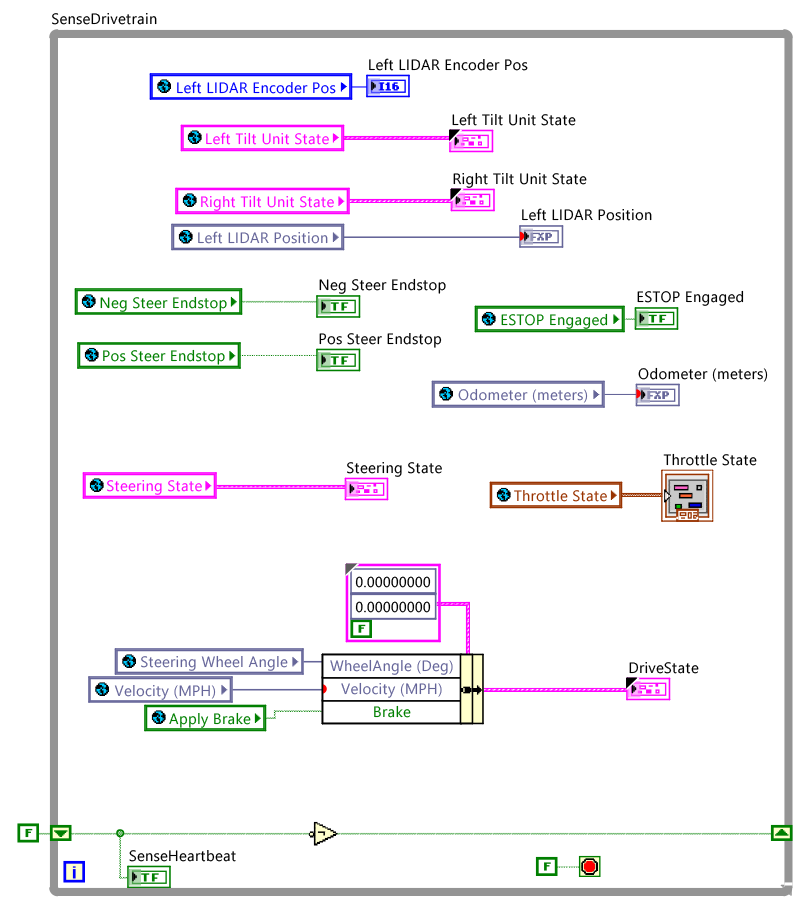
\includegraphics[scale=1.5]{Photos/sensingloop.png}
\caption{Sensing loop in the hindbrain VI}
\label{fig:sensingloop}
\end{figure} 

\noindent As shown in Figure \ref{fig:sensingloop}, the sensing loop is responsible for exposing front panel elements for the following pieces of data to the real-time code:

\begin{enumerate}
\item Left LiDAR Encoder Position: A debugging indicator that shows the encoder position of the left LiDAR in units of encoder ticks
\item Left Tilt Unit State: A cluster containing an indicator for whether the index had been found, whether the tilt unit has been told to be in initialize mode, whether there is a position error in the tilt unit and the encoder position.
\item Right Tilt Unit State: The same cluster as the left tilt unit state cluster used for the right tilt unit
\item Left LiDAR Position: Another debug indicator that shows the position of the left tilt unit in degrees after the encoder ticks have been converted to degrees
\item Negative Steer Endstop: A boolean that represents whether the negative steer angle endstop has been triggered
\item Positive Steer Endstop: A boolean that represents whether the positive steer angle endstop has been triggered
\item Estop Engaged: A boolean that represents whether either of the physical estop buttons have been triggered
\item Odometer (meters): The distance travelled by the vehicle since the code started running
\item Throttle state: A cluster containing indicators for the gas and brake pedal voltage being sent to the linear actuators for the gas and brake respectively
\item DriveState: A cluster indicating the driving state of the vehicle including the steering wheel angle in degrees, the velocity in miles per  hour and the boolean that represents whether the vehicle should apply the brakes
\item SenseHeartBeat: An indicator that simply provides a blinking light that confirms the while loop is running 
\end{enumerate}

\subsection{Acting Loop}

The acting loop of the FPGA hindbrain essentially performs the opposite function of the sensing loop: to provide indicators for the real-time code to pass commands or instructions down to the FPGA code. The block diagram for the acting loop shown in Figure \ref{fig:hindbrainblock} is shown zoomed in below:

\newpage

\begin{figure}[h!]
\centering
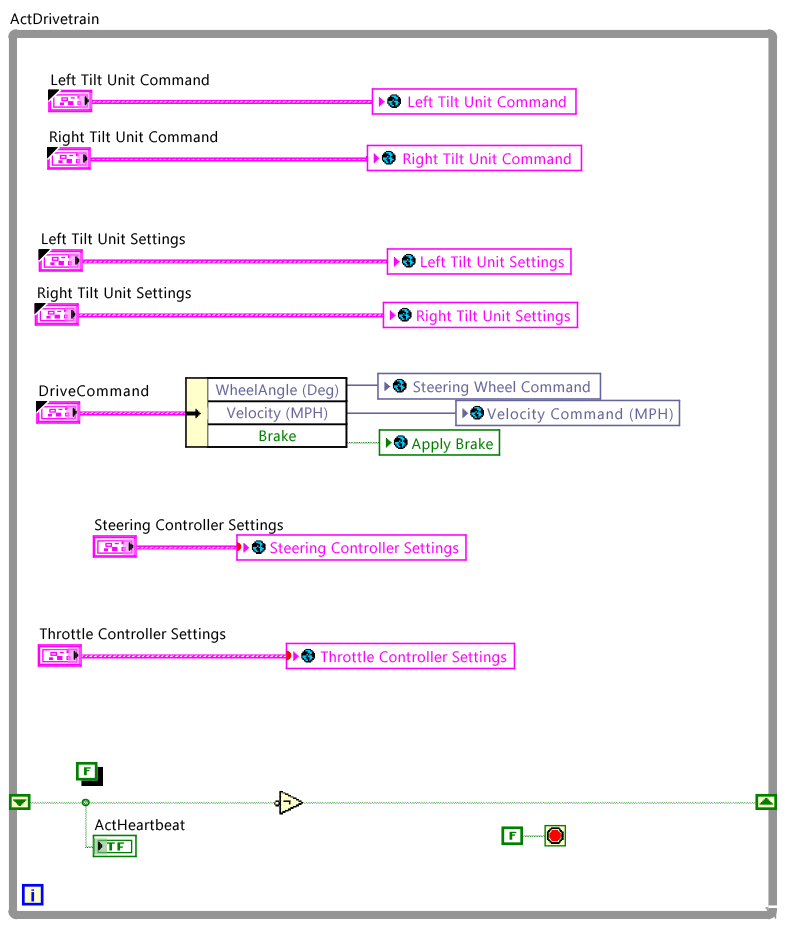
\includegraphics[scale=1.5]{Photos/actloop.png}
\caption{Acting loop in the hindbrain VI}
\label{fig:actloop}
\end{figure}

\noindent As shown in Figure \ref{fig:actloop}, the acting loop is responsible for providing front panel elements for the real-time code to send the following commands to the FPGA code:

\begin{enumerate}
\item Left Tilt Unit Command: A cluster that contains indicators for whether the tilt unit should be in initialize mode, the position setpoint of the tilt unit in degrees, the current output when the tilt unit is in initialize mode and a reset position boolean that indicates whether the position of the tilt units should be reset to zero.
\item Right Tilt Unit Command: The same cluster as Left Tilt Unit Command, but for the right tilt unit
\item Left Tilt Unit Settings: A cluster that contains the controller settings for the left tilt unit including the position proportional, integral and derivative (PID) gains, Current PI gains and the current limit
\item Right Tilt Unit Settings: The same settings cluster as the Left Tilt Unit Settings for the right tilt unit
\item Drive Command: A cluster containing the desired wheel angle in degrees, the desired velocity in miles per hour and a boolean to command the vehicle to apply the brakes
\item Steering Controller Settings: A cluster containing the controller settings for the steering control including the PID gains, upper and lower voltage limits, upper and lower encoder limits, PID to motor conversion constant, motor deadband high and low threshold, a reset position boolean for resetting the steer motor position and two other booleans to tell the vehicle whether to allow positive and negative steering voltages or not.
\item Throttle Controller Settings: Cluster containg the throttle controller settings for the gas and brake controllers including the PID gains for the gas pedal controller, voltage offset that indicates the neutral position voltage, position reset and PID reset boolean, maximum and minimum brake voltage, maximum and minimum gas pedal voltage and the speed of the throttle control loop. 
\end{enumerate}

\subsection{Tilt Unit Drive Status Monitors}
The tilt unit drive status monitors essentially provide inputs and outputs that allow the real-time code to command the NI9505 motor control modules and receive information on the status of the modules. The block diagram for the tilt unit drive status monitors shown in Figure \ref{fig:hindbrainblock} is shown zoomed in below

\newpage

\begin{figure}[h!]
\centering
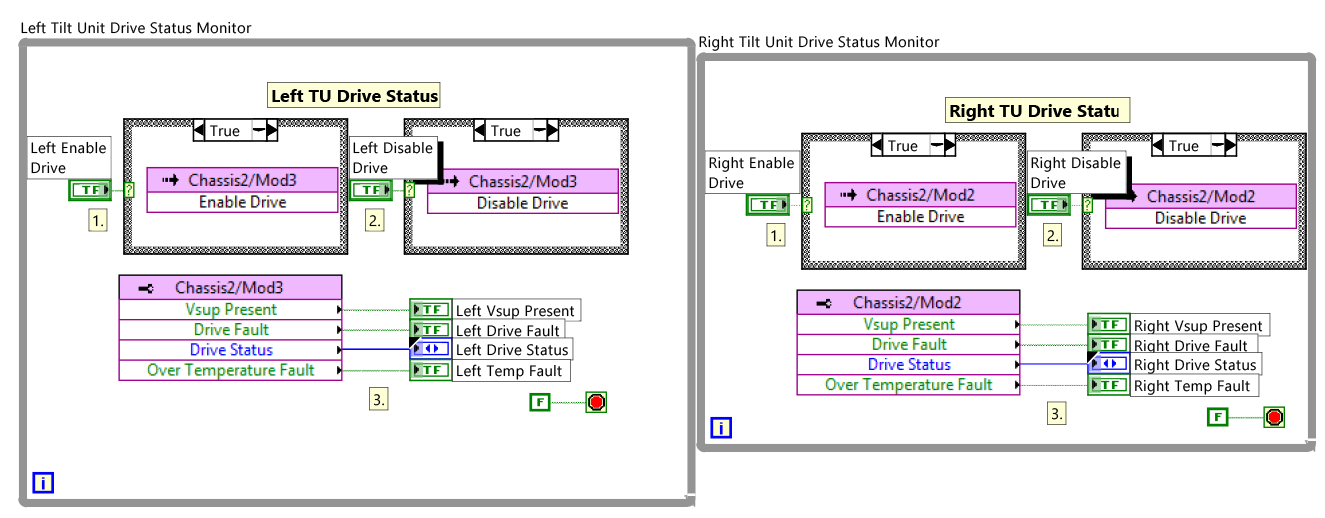
\includegraphics[scale=1.2]{Photos/tudrivestat.png}
\caption{Tilt unit drive status monitors in the hindbrain VI}
\label{fig:tudrivestat}
\end{figure}

\noindent As can be seen in Figure \ref{tudrivestat}, the left and right drive status loops are basically identical to each other except for the module assignments since the left drive status monitor addresses the NI9505 module for the left tilt unit and the right drive status monitor addresses the other NI9505 module. \\ \\
%
Each drive status monitor loop contains a method for enabling the drive, disabling the drive and monitoring the presence of a power supply (vsup Present), whether the drive has a drive fault (Drive Fault), determining whether the drive is enabled or disabled (Drive Status) and whether the drive is overheating (Over Temperature Fault). By default, the NI9505 modules will be disabled when the vehicle is first powered up and so the drive will need to be enabled in software during initialization. 

\subsection{LiDAR Reading}

Although LiDAR reading shows up on the front panel of the Hindbrain top-level VI as one subVI, the process of reading data from the two Sick LMS291 LiDARs really involves several different subVIs to perform the various tasks. In summary, the process of reading data from the LiDARs involves:

\begin{enumerate}
\item Initializing the LiDARs
\item Read the raw data from the LiDARs
\item Parse and transform the LiDAR data into the vehicle's coordinate system
\end{enumerate}

\noindent On the hindbrain top-level VI, the block diagram for reading the LiDARs shown in Figure \ref{fig:hindbrainblock} is shown zoomed in below:

\begin{figure}[h!]
\centering
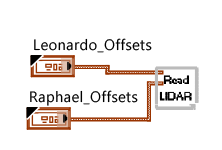
\includegraphics[scale=2]{Photos/lidarread.png}
\caption{LiDAR Reading SubVI in the hindbrain VI}
\label{fig:lidarread}
\end{figure}

\noindent As can be seen in Figure \ref{fig:lidarread}, the lidar reading VI takes the offsets for the left (Leonardo) and right (Raphael) LiDARs that provide the translations and rotations that are needed to transform the LiDAR data in the last step of the LiDAR reading process.\\ \\
%
The block diagram of the LiDAR reading VI is shown below:

\begin{figure}[h!]
\centering
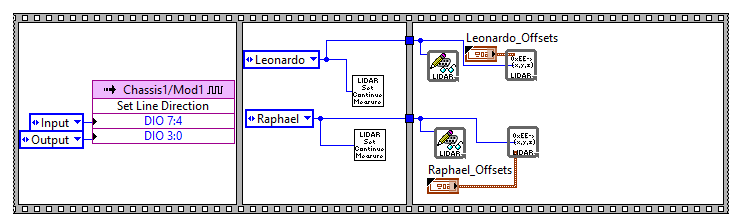
\includegraphics[scale=0.75]{Photos/readlidarblock.png}
\caption{Block diagram for the Lidar Reading VI}
\label{fig:readlidarblock}
\end{figure}

\noindent As can be seen in Figure \ref{fig:readlidarblock}, the LiDAR reading VI consists of a flat sequence with three parts:

\begin{enumerate}
\item The first part is an FPGA I/O method node that sets the the input and output lines
\item The second part contains a VI for the left and right LiDAR that sends the commands specified in the LiDAR communication protocol to tell the LiDAR to send data continuously at 25Hz
\item The third part contains two subVIs: a serial read/write VI that writes the required commands to the LiDAR and receives the LiDAR data back and a transformer VI that transforms the LiDAR data coordinate system from the LiDAR's local coordinate system to the vehicle's coordinate system.
\end{enumerate}

\subsection{LiDAR Serial Read/Write}

The block diagram for the LiDAR serial read/write VI is shown below:

\begin{figure}[h!]
\centering
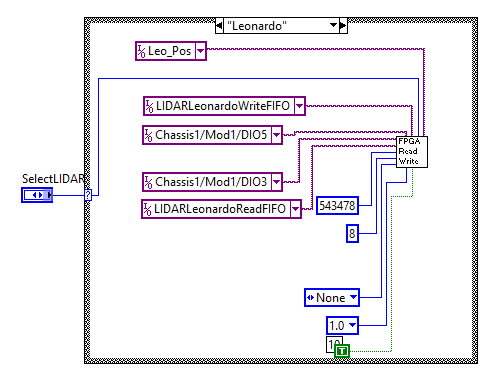
\includegraphics[scale=0.75]{Photos/readlidar_block.png}
\caption{Block diagram for the Lidar Reading VI}
\label{fig:readlidar_block}
\end{figure}

\noindent As can be seen in Figure \ref{fig:readlidar_block}, the VI is essentially a wrapper for the actual FPGA read/write functions that allows the code to reuse the same read/write functions while being able to assign the inputs and outputs to the appropriate LiDARs (either left or right). The VI takes either the left (Leonardo) or right (Raphael) LiDAR name as input and assigns the following variables to the write function:

\begin{enumerate}
\item LIDARLeonardoWriteFIFO: A First In First Out (FIFO) queue that queues the LiDAR commands to be sent to the LiDAR 
\item Chassis1/Mod1/DIO3: The DIO chanel from which LiDAR data is transmitted
\item 543478: The baud rate for LiDAR communication
\item 8: Data bits for the LiDAR
\item None: Parity for the LiDAR
\item  1.0: Stop bits
\item True boolean: Reverse Polarity command for the LiDAR
\end{enumerate}

\noindent The read function is then assigned the following variables:

\begin{enumerate}
\item LeoPos: A FIFO queue that queues the lidar position data to be read by the transformer VIs
\item Chassis1/Mod1/DIO5: The DIO channel from which LiDAR data is received
\item LIDARLeonardoReadFIFO: THe FIFO queue that queues the received LiDAR data
\item 543478: The baud rate for LiDAR communication
\item 8: Data bits for the LiDAR
\item None: Parity for the LiDAR
\item  1.0: Stop bits
\item True boolean: Reverse Polarity command for the LiDAR
\end{enumerate}

\noindent These variables are then passed down to the actual serial write and read functions as shown below:

\newpage

\begin{figure}[h!]
\centering
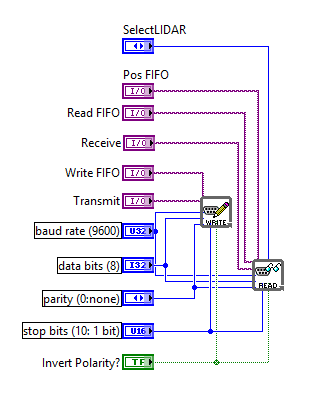
\includegraphics[scale=0.75]{Photos/readwriteblocks.png}
\caption{Block diagram for the VI providing the actual read/write functions}
\label{fig:readwriteblocks}
\end{figure}

\noindent The serial write VI is a stock serial write VI provided by LabVIEW for the LiDARs that has been modified to include a while loop around the entire serial write sequence for the LiDARs. Therefore, for brevity in this report, the write VI will not be explained in detail. However, for convenience, the documentation for the serial write VI is shown in the figure below:

\begin{figure}[h!]
\centering
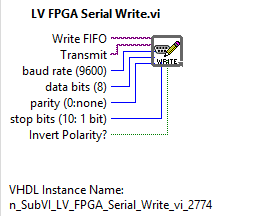
\includegraphics[scale=0.75]{Photos/writedocs.png}
\caption{Documentation for the serial write function}
\label{fig:writedocs}
\end{figure}

\newpage

\noindent The block diagram for the serial read VI, then, is shown in the diagram below:

\begin{figure}[h!]
\centering
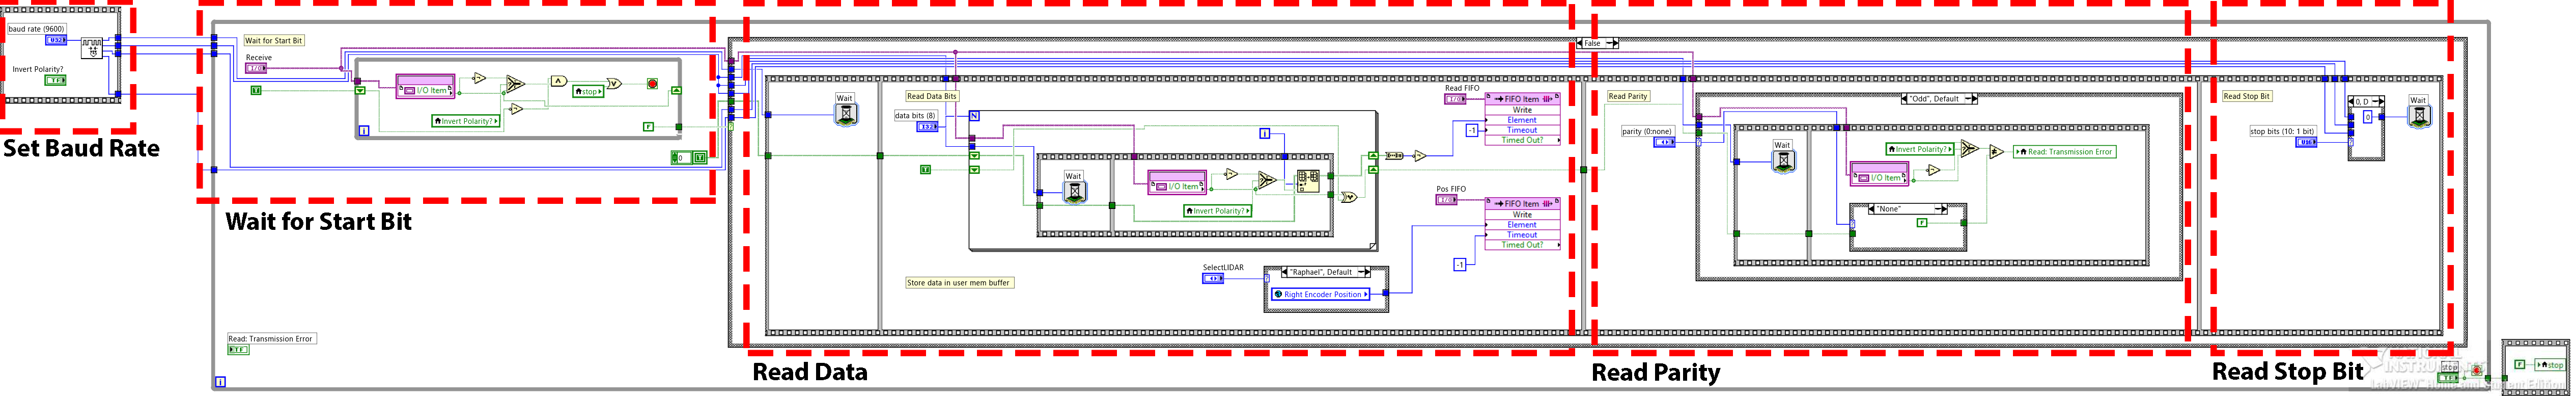
\includegraphics[scale=0.35]{Photos/serialreadblock.png}
\caption{Block diagram for the serial read function}
\label{fig:serialreadblock}
\end{figure}

\noindent As can be seen in Figure \ref{fig:serialreadblock}, after setting the baud rate, the VI executes a series of steps each time throug the while loop to receive the bits that make up the LiDAR data that is received:

\begin{enumerate}
\item Wait for the start bit of the data
\item Read data
\item Read stop bit
\end{enumerate}

\noindent For brevity, this report is not going to discuss the code that waits for the start bit or the code that reads the stop bit. When zoomed in, the read data chapter of the code is as follows:

\begin{figure}[h!]
\centering
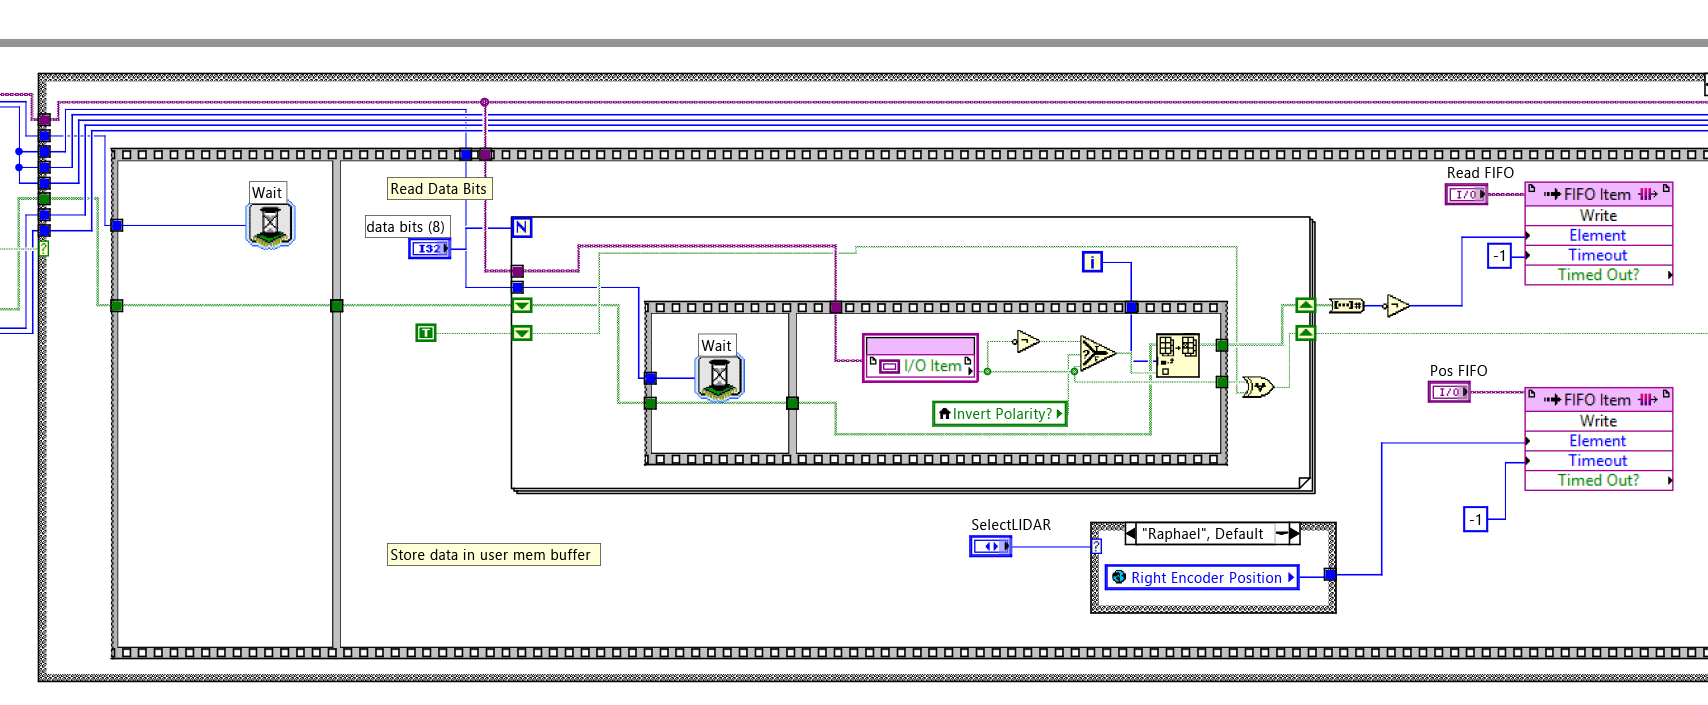
\includegraphics[scale=0.85]{Photos/readdatasection.png}
\caption{Block diagram for the chapter that reads the LiDAR data bits}
\label{fig:readdatachapter}
\end{figure}

\newpage

\noindent As can be seen in Figure \ref{fig:readdatachapter}, the data reading code essentially reads each bit as a boolean and adds it to the array. Once the for loop has been through all the bits in the mesage, it converts it to a number and adds the number to the read FIFO queue that queues up the LiDAR reading to be read by the transforming code. At the same time, code in parallel reads either the left or right encoder position (depending on whether Raphael or Leonardo is selected) and and appends the encoder tick count to a separate position FIFO queue to be read by the transformer code.

\subsection{LiDAR Data Transform}
Referring back to Figure \ref{fig:readlidarblock}, after the LiDAR read/write functions, the next step in processing the LiDAR data is to transform it from the local LiDAR coordinate system to the vehicle coordinate system. 

\subsubsection{Overview of the Transform Process}

The data returned by the Sick LMS290 LIDARs is in the co-ordinate frame of the LIDARs by virtue of the way in which the LIDARs take readings. In order to do useful work with the LIDAR data, the LIDAR data has to be transformed to make it iwth reference to the vehicle co-ordinate system. \\ \\
%
\noindent The transform process has three parts:

\begin{enumerate}
\item Convert each scan from polar co-ordinates to cartesian co-ordinates
\item Rotate the coordinate frames such that the frame local to the LIDAR is in the same orientation as the vehicle co-ordinates
\item Translate the coordinate frames such that the frame local to the LIDAR is translated to line up with the vehicle co-ordinate system
\end{enumerate}

\subsubsection{Constant LIDAR Transform Properties}
Based on the design and placement of the LIDAR mounts, the following properties of the LIDAR transform to t